\chapter{Project Objectives}\label{ch:obiective}
\pagestyle{fancy}

The main focus of this thesis is to create a hardware-accelerated Digital Twin, called \textit{ChronoLux}, which will provide an interactive and physically-based lighting simulation for the conservation of cultural heritage. This solution is designed to fill the important missing link between computationally-heavy offline rendering systems (such as Radiance), which can be proven mathematically, and real-time IoT sensing devices.

In order to achieve this high-level goal and provide the necessary combination of interactivity and scientific accuracy, the development process is carried out based on certain technical and metrological goals. The high-level architecture related to these goals is outlined in Figure \ref{fig:concept_diagram}.

\section{Technical and Architectural Objectives}

\begin{enumerate}[label=\textbf{O\arabic*.}]
    \item \textbf{Texture Space Ray Tracing Integration:}
          To address the drawbacks associated with traditional screen space algorithms, such as frustum culling that results in critical out-of-screen lighting information being removed from calculations, a special compute shader for DirectX 12 Raytracing (DXR) would have to be used to launch rays directly from the unwrapped UV texture map of 3D models in order to permanently bake the cumulative radiometric energy into all of its geometric surface regardless of the location of the observer.

    \item \textbf{Physical Environmental Modeling:}
          In order to combine the Perez All-Weather Sky Model with a special Next Event Estimation (NEE) compute algorithm to create a scientifically rigorous method to decouple the direct beams of sunlight from the diffuse ambient lighting, thus generating physically correct global illumination without loss of real-time processing ability.

    \item \textbf{Asynchronous Compute Architecture:}
          For a proper separation of concerns between the user interface layer and computationally demanding GPU path tracing engine, the program should allow users to modify physical properties (transmission coefficients of window glazing or wall reflectance, for instance) via an interactive UXML/USS user interface without breaking the continuity of the 60 FPS viewport interaction.

\end{enumerate}

\section{Metrological and Validation Objectives}

\begin{enumerate}[label=\textbf{O\arabic*.}]
    \setcounter{enumi}{3}

    \item \textbf{Headless Statistical Telemetry:}
          In this study, an automated approach has been developed for virtual point-probe Lux sensors which operate purely in the background. The sensors are created for the purpose of computing spatial variance ($\sigma^2$), maximum exposure dose, and standard Monte Carlo convergence error boundaries while not interfering with the primary rendering process.

    \item \textbf{Empirical Scenario Validation:}
          Explicit validation of the above approach is achieved by means of running simulations of an entire year of meteorology (i.e., 8,760 hours of continual processing) for various preventive conservation scenarios. It is essential for establishing the efficacy of dynamic environmental control actions like the application of UV-absorbent windows or optimizing geometric occlusion of susceptible artworks.

\end{enumerate}

\begin{figure}[h]
    \centering
    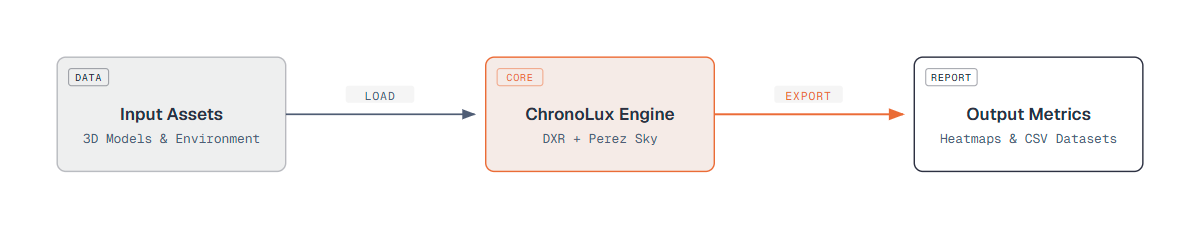
\includegraphics[width=1\textwidth]{figures/concept_diagram.png}
    \caption{High-Level Concept Architecture of the ChronoLux framework, illustrating the pipeline from raw heritage asset ingestion to real-time dosimetric data export.}
    \label{fig:concept_diagram}
\end{figure}

The subsequent chapters of this thesis will methodically detail the design, theoretical foundation, programmatic implementation, and scientific validation of these stated objectives.
